\section{波场外推的物理问题与修饰处理问题}
\label{sec:4.1}

频率滤波、倾角滤波以及增益控制看来是目的在于进行大量修饰的三种处理:它们全都
是用于改善地震记录面貌。选择这些处理或类似处理的定量参量时所采用之准则往往是含糊
不清的,而且与人的经验或视觉有关。原则上,乞灵于信息论并采用像信号与噪音倾角普之
类的客观准则,应该有可能选出所需的参量,但是在常规的实际工作中,迄今还没这样作
过。

不应当低佶修饰性处理的重要性,例如,想对一些处理技术方法进行比较,在许多场合
下往往就因为修饰性参量发生意外的变化,而导致失败。要求有这些修饰性处理是在波动传
播理论内自然而然产生的,所以,看来最好是首先理解它们是如何形成的,然后在处理过程
中进行这些修饰,而不要在处理以后才试图以某种人为方式生硬地附加上去。现在将对波场
外推方程各个部分逐一加以研究,以指出它们的修饰性效果。



\subsection{$t$平方函数}
\label{sec:4.1.1}

反射随时间而变弱。为能看清较晚时间到达的数据,我们一般要使数据的放大倍数随时
间而增大。我始终很少因我选取$t^2$函数作为比例因子而感到失望过。不可能总是期望产比例
函数行得通,因为它到底是以非常简单的模型为基础的。但是我发现$t^2$比流行的抉择、即选
取增长指数函数,更令人满意。$t^2$函数没有什么参量,而指数函数则要求有两个参量,一个
是时间常数,另一个是截止时间,也就是到达这个时间你必须停止指数增长,因为它会变得
过于大了。

$t$取二次幂有两个原因。第一个原因是因为我们正在把三维问题变换为一维问题。地震
波是在三维空间内扩展的,不断扩展着的球面波阵面表面面积与半径之平方呈正比关系,因
而能量分布面积隨时间之平方而正比增大:但是地震波振幅是与能量之平方根成比例的,所
以由能量分布的这种基本几何形态关系可预言球面发散校正仅需时间的一次幂。

第二个原因是由计算简单的吸收而引起。讨论吸收作用要有某种模型,我将提出的模型
对于解释有关地震波吸收的任何事情都显得过于简单了,可是它却能很好地预言应有另一个
时间的一次幂,而经验证明我们确实是需要如此。关于该模型,我们假设:
\begin{enumerate}

\item
  一维空间传播;
\item
  速度恒定;
\item
  吸收Q\textsuperscript{-1}为恒定;
\item
  反射系数沿深度方向为随机的;
\item
  不存在多次反射;
\item
  震源为白噪音。
\end{enumerate}

这些假设直接告诉我们:单频波将随深度而指数式衰减,比如说,按$exp(-\alpha \omega t)$而
衰减,其中$t$为旅行时间深度,$\alpha$为与波动品质因数Q呈反比关系的衰减常数。在人们用这样
一种单频波来模拟真实的地震数据的时候,许多人都会误入岐途。比较好的一种模型是采用
宽频带的地震震源,例如采用脉冲函数。因为有吸收作用,高频分量衰减很迅速,最终只剩
下低频分量,因而较低频率的信号得到增强。在传播时间为$t$时,原来的白噪谱(常数谱)
为前面提到的频率之阻尼指数函数$exp(-\alpha\omega t)$所代替。形成脉冲时间函数所需的能量仅
与该频率的阻尼指数函数之下的面积是成比例的。至于说到相位,因为是假设脉冲震源而
且速度是假设为常数,所有频率成分均将是同相的(见\ref{sec:4.6}节关于因果性问题的讨论)。将
该指数函数从零至无限大频率进行积分,使我们得到负一次幂的时间$t^{-1}$,从而完成了发散
校正应为$t^2$的证明。

奇怪的是预期的地震记录包络$t^2$的形状并不依赖于耗散常数$\alpha$,但是改变地震震源的谱
的确会改变包络的形状。这里作为一个习题留待读者去征明:地震震源具有形式为$\mid \omega \mid^\beta$的
谱,其含意就是发散校正因子应为$t^{2+\beta}$。

地震波速度随深度而增大,所以知道速度的人有时可使校正因子既是时间的(因而是炮
检距的)、也是速度的一个函数,从而可能使发散校正得到改善。

在实际工作中,运气好也许产能良好地拟合于数据。实际上,Q值一般是随深度而增
大,而反射系数一般是随深度而减小。

\subsection{噪音、面波与限幅}
\label{sec:4.1.2}

如果地震数据除了反射没包含别的,这时要显示它不会有什么麻烦。你大概会直接乘以
$t^2$,然后进行标定使得最大的数据值也能保持在有效显示区域内。在实际处理工作中存在有两
个问题:(1)干扰记录道;(2)噪音传播方式。之所以会有干扰记录道,是因为世上人们
的活动不会全是静止的,从而形成了一些干扰;噪音传播方式是指波被封闭在表面地层内的
情形。所以,它们的发散要在二维空间内考虑,而不是像反射那样在三维空间内考虑。海水
层干扰额外地强,因为水层具有均匀性而且吸收作用很低。

对于噪音要按低于极大值的某科水平对数据值进行限幅(clipping)的办法来加以处
理。限幅的意思就是把大于限幅值的各个值均用限幅值来代替。由于噪音的大小一般是不可
预测的,最可靠的方法应该是采用分位数(quantile)。试想象把数据的采样值根据其绝对
值的大小按数值顺序加以分类。将第n分位数$n^{th}$定义为是这样的绝对值:它等于最大绝对值
与最小绝对值之差的$n/100$。如果按百分位数(percenfile)$99^{th}$将数据加以限幅,则多达
百分之一的数据可以是无限强的噪音。我发现大多数野外剖面受干扰采样值的数量都小于
$10\%$,所以我经常两次采用百分位数$90^{th}$作限幅。要求出分位数,没必要将数据全部分类,
那样作就太慢了,可以采用牧速得多的Hoare算法(欲知详倩和更多地球物理方面的应用,
可参阅“地球物理数据处理基础”一书或者Claerbout与Muir(l973)的论文)。

不同的显示具有不同的目的。重要的往往是在进行处理过程中保持线性性质,但是在最
后阶段一一即显示时可以牺牲线性性质以便使我们能够观察到所有强的和弱的同相轴。
人类的感觉作用一般来说毕竟是符合对数律的。在我们的实验室中,我们一般是采用乘幂
律。我发现以其带正负号的平方根值来代替数据采样值本身一般是可将所有信号均压缩为某
种可见域的。在显示具有非常小的记录道间距之野外剖面时,可能最好是采用带正负号的立
方根值。更一般性地说,我们可采用具有下列关系的非线性增益
\begin{equation}
\text{显示}=sgn(\text{数据}\mid\text{数据}\mid^{\gamma})
\label{eq:ex4.1.1}
\end{equation}
式中,伽马$\gamma$是摄影术中用以描述摄像胶片之非线性程度的一种专门术语。本书中大多数的数
据图形是采用$\gamma=1$以及$t^2$增益,而且按百分位数$99^{th}$限幅。

工业应用的标准办法看来是自动增益控制AGC。自动增益控制AGC的意思是对某稗间
隔内的数据幅度取平均,然后再除以幅度。尽管AGC是非线性的,可是它出采甩$\gamma$值更接近
于线性关系,所以当你计划以后的处理时,采用它大概是比较好的。不过,利用AGC时,
你就失去了可逆性以及绝对增益的感觉。

图\ref{fig:dspr/agc}是个有趣的例子。由于它是个中间放炮排列,你也许推测它是陆地资料,船是
不可能将电缆在船的前面推着走的。但是,左图清清楚楚是表示海上的多次波,混响的周期
是均匀的,而且在海底反射之前没有其俾反射。它必然是在覆盖深水(375米)的冰层上面
所采集的资料。从采用非线性增益的中图我们可清晰地看出有一海水层的波,而在它之前有
速度较快的泳层内之波。图中也有冰面上较微弱的低速低频“地滚波”,还有一些良好的反
射。

\begin{figure}[H]
\centering
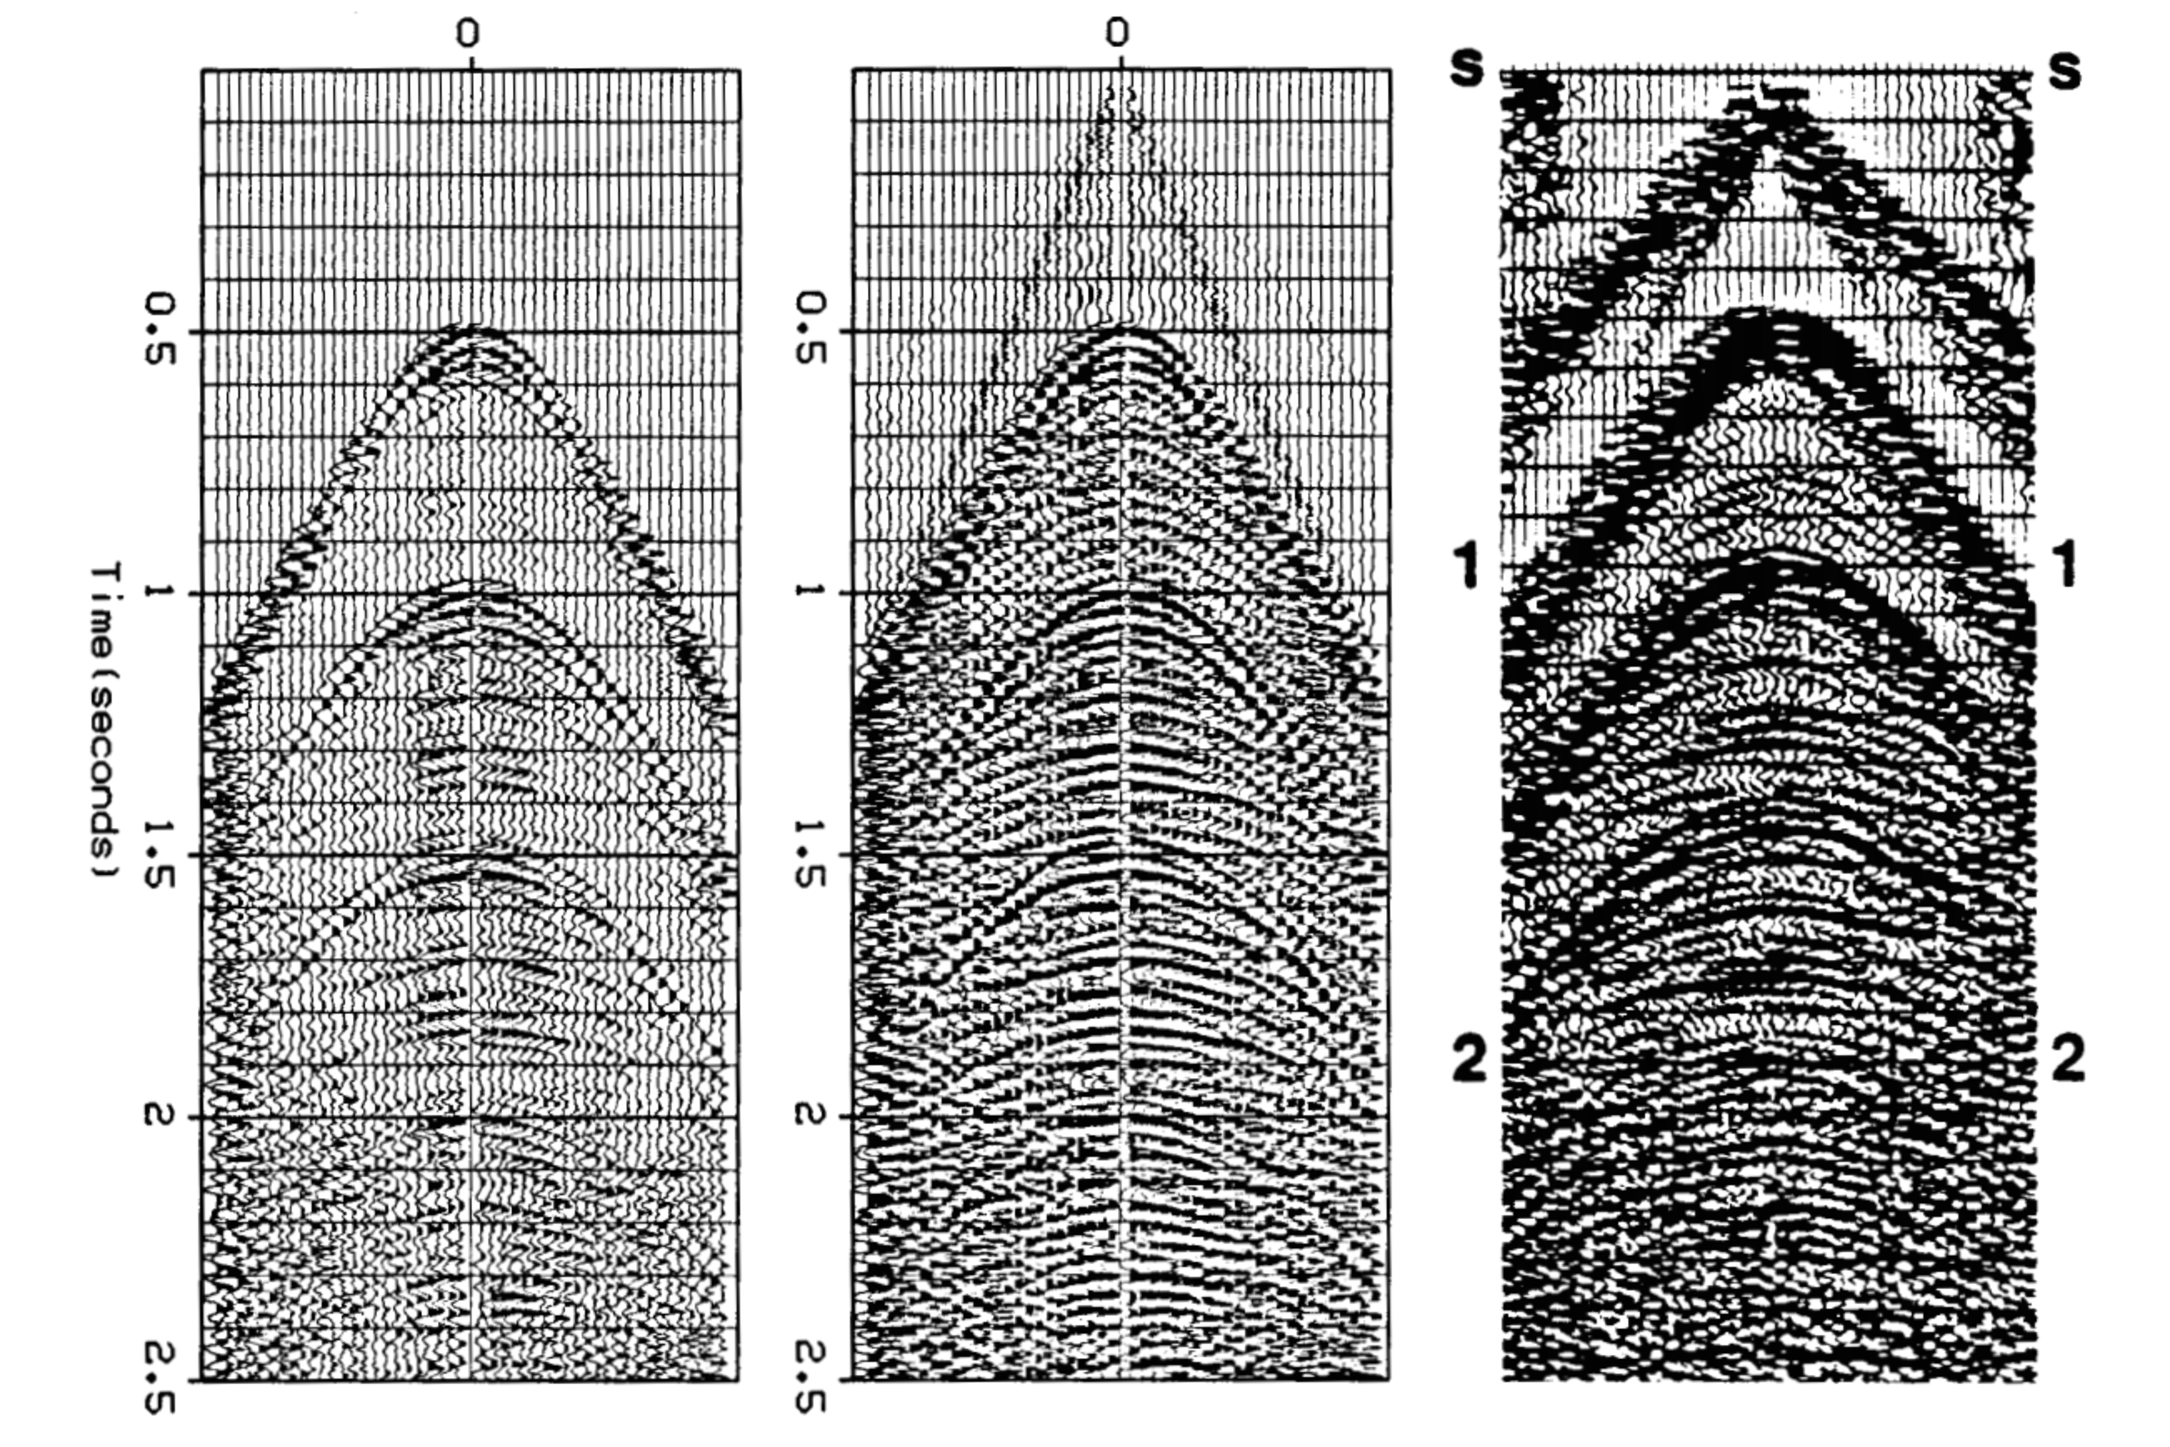
\includegraphics[width=0.65\textwidth]{dspr/agc}
\caption[agc]{西方地球物理公司提供的北极地区记录剖面。左图,采用$t^2$增益。中图,
采用$t^2$增益和$\gamma=0.4$。右图,采用西方地球物理公司的AGC增益}
\label{fig:dspr/agc}
\end{figure}


\subsection{$5^{\circ}$近似方程中的复速度}
\label{sec:4.1.3}

5°近似方程,即
\begin{subequations}
\begin{equation}
\frac{\partial P}{\partial z}=\frac{1}{v}\frac{\partial P}{\partial t}
\label{eq:ex4.1.2a}
\end{equation}
\begin{equation}
ik_z=-\frac{i\omega}{v}
\label{eq:ex4.1.2b}
\end{equation}
\label{eq:ex4.1.2}
\end{subequations}
表明一个波阵面要取若干时间才能从一个深度传播到另一个深度。因速度$v$为实常数,由式
\ref{eq:ex4.1.2}所描述的各波在传播中均不改变其形状。在实际工作中,总观察到有波形变化,
所以,$v$不应该是一个实常数。速度的虚部将形成衰减,速度与频率有关将引起频散。

\subsection{吸收作用}
\label{sec:4.1.4}

当速度$v(\omega)$按下述方程定义时
\begin{equation}
-\frac{i\omega}{v(\omega)}=\frac{\omega_0}{v_0}(-\frac{i\omega}{\omega_0})^{1-\epsilon}
\label{eq:ex4.1.3}
\end{equation}
就产生了吸收作用的基本模型。在$\epsilon =
0$时,方程\ref{eq:ex4.1.3}给出常速度。在\ref{sec:4.6}节中将证明,
方程\ref{eq:ex4.1.3}是模拟所谓的因果性恒定Q值阻尼衰减,此处,$Q^{-1}=\tan \pi\epsilon$。图\ref{fig:dspr/qhale}所示
是利用式\ref{eq:ex4.1.2}和\ref{eq:ex4.1.3}按爆炸反射面模型作出的合成地震记录。

\begin{figure}[H]
\centering
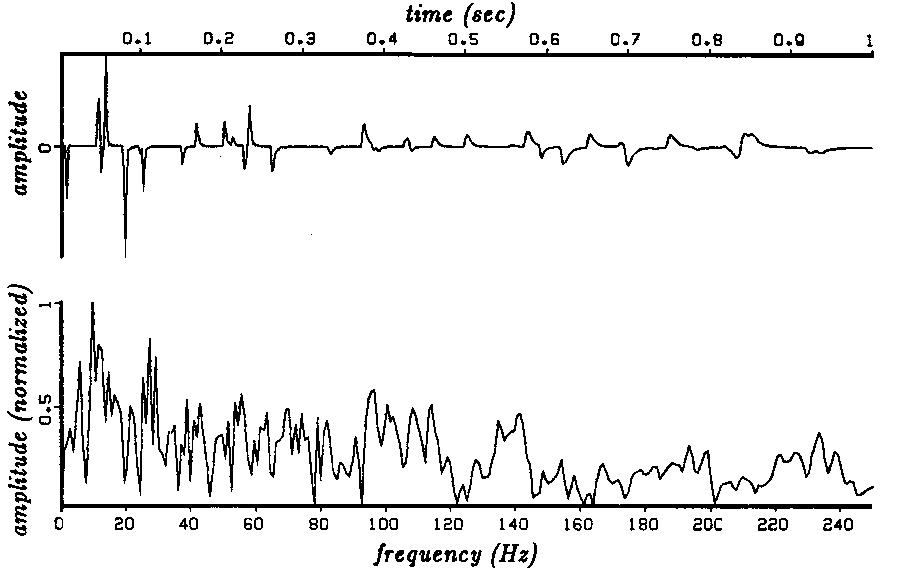
\includegraphics[width=0.65\textwidth]{dspr/qhale}
\caption[qhale]{地层Q值为$Q=100$时的合成地震记录(据Hale)}
\label{fig:dspr/qhale}
\end{figure}

式\ref{eq:ex4.1.3}在速度中引入了虚部,因而形成衰减,这种衰减的主要影响就是使到达时间
晚的初至削弱。第二种影响就是使晚到之初至的频率成分变低。第三种影响则是这样:它之
所以出现是由于因果性条件的要求迫使速度的实部或多或少地与频率有关。在图\ref{fig:dspr/qhale}中,
各个脉冲的“上升时间”均比“下落时间”(fall
time)要快,就是证实有这种稍微与频
率有关的现象。这种现象意味着高频成分的传播比低频成分稍微快一些。在实际工作中,这
第三种影响非常值得注意。

实现地层成像时,在向下延拓期间放大高频能量,就能够补偿掉地层耗散作用。这种补
偿处理除了要以像$ik_z=(-i\omega)^{1-\epsilon}$这种项代替$k_z=\sqrt{k_x^2-\omega^2/v^2}$之外,几乎就能够像偏移一
样来完成。不过,由于它会把噪音放大,实际上并没有人愿意这样作。所以,这就产生了信
噪比的问题。 

噪音并非简单就是环境背景的随机起伏,如重复放炮,它多半是可重复出现的。噪音是
迄今我们还没法提出满意机制模型的一种东西。按照目前的实际处理水平,往往习惯于采用
时变滤波来选择中意的时变通带。方程\ref{eq:ex4.1.2}与\ref{eq:ex4.1.3}能够用于实现这种时变滤波,
不过要是把它们的使用看成就是补偿地层Q值变化,却是过于简单化了。

\subsection{频散作用}
\label{sec:4.1.5}

在有面波存在的情形下,速度对频率的依赖关系是极明显的。例如,速度对频率的依赖
关系由下述方程给出
\begin{equation}
-\frac{i\omega}{v(\omega)}=-\frac{i\omega}{v_0}\sqrt{1+\omega_0^2/\omega^2}
\label{eq:ex4.1.4}
\end{equation}
图\ref{fig:dspr/sword}(a)包含有某种频散地滚波。在图\ref{fig:dspr/sword}(b)中,采用类似偏移的处理,该频散现
象就消除了。这种处理同偏移处理之间的一种差别就是:偏移是沿$z$轴向下外推,而在图
\ref{fig:dspr/sword}(b)中则是沿x轴外推(实际上,外推方向都只是在计算机内处理的)。在图\ref{fig:dspr/sword}
(左图)中,每个记录道都是单独处理。在偏移方法中,利用频散关系$k_z=-\sqrt{\omega^2/v^2-k_x^2}$
将数据$p(t,z=0)$外推为映象$p(t=0,z)$;在图\ref{fig:dspr/sword}(左图)的处理中,则是利用像
$k_x=f(\omega/v)$的这类频散关系将数据$p(t,x=0)$外推为映象$p(t=0,x)$。在完成这种赝偏移
(pseudomigration)之后,再用常速作廣绕射扫描(pseudodiffraction),其总效果就是
消除频散,最终就有可能看出,干扰原来是由两种独立的同相轴组成的。

类似这样一种处理技术曾经首先应用于探测煤层中的断层(Beresford-Smith与Mas-on, 1980年)。

\begin{figure}[H]
\centering
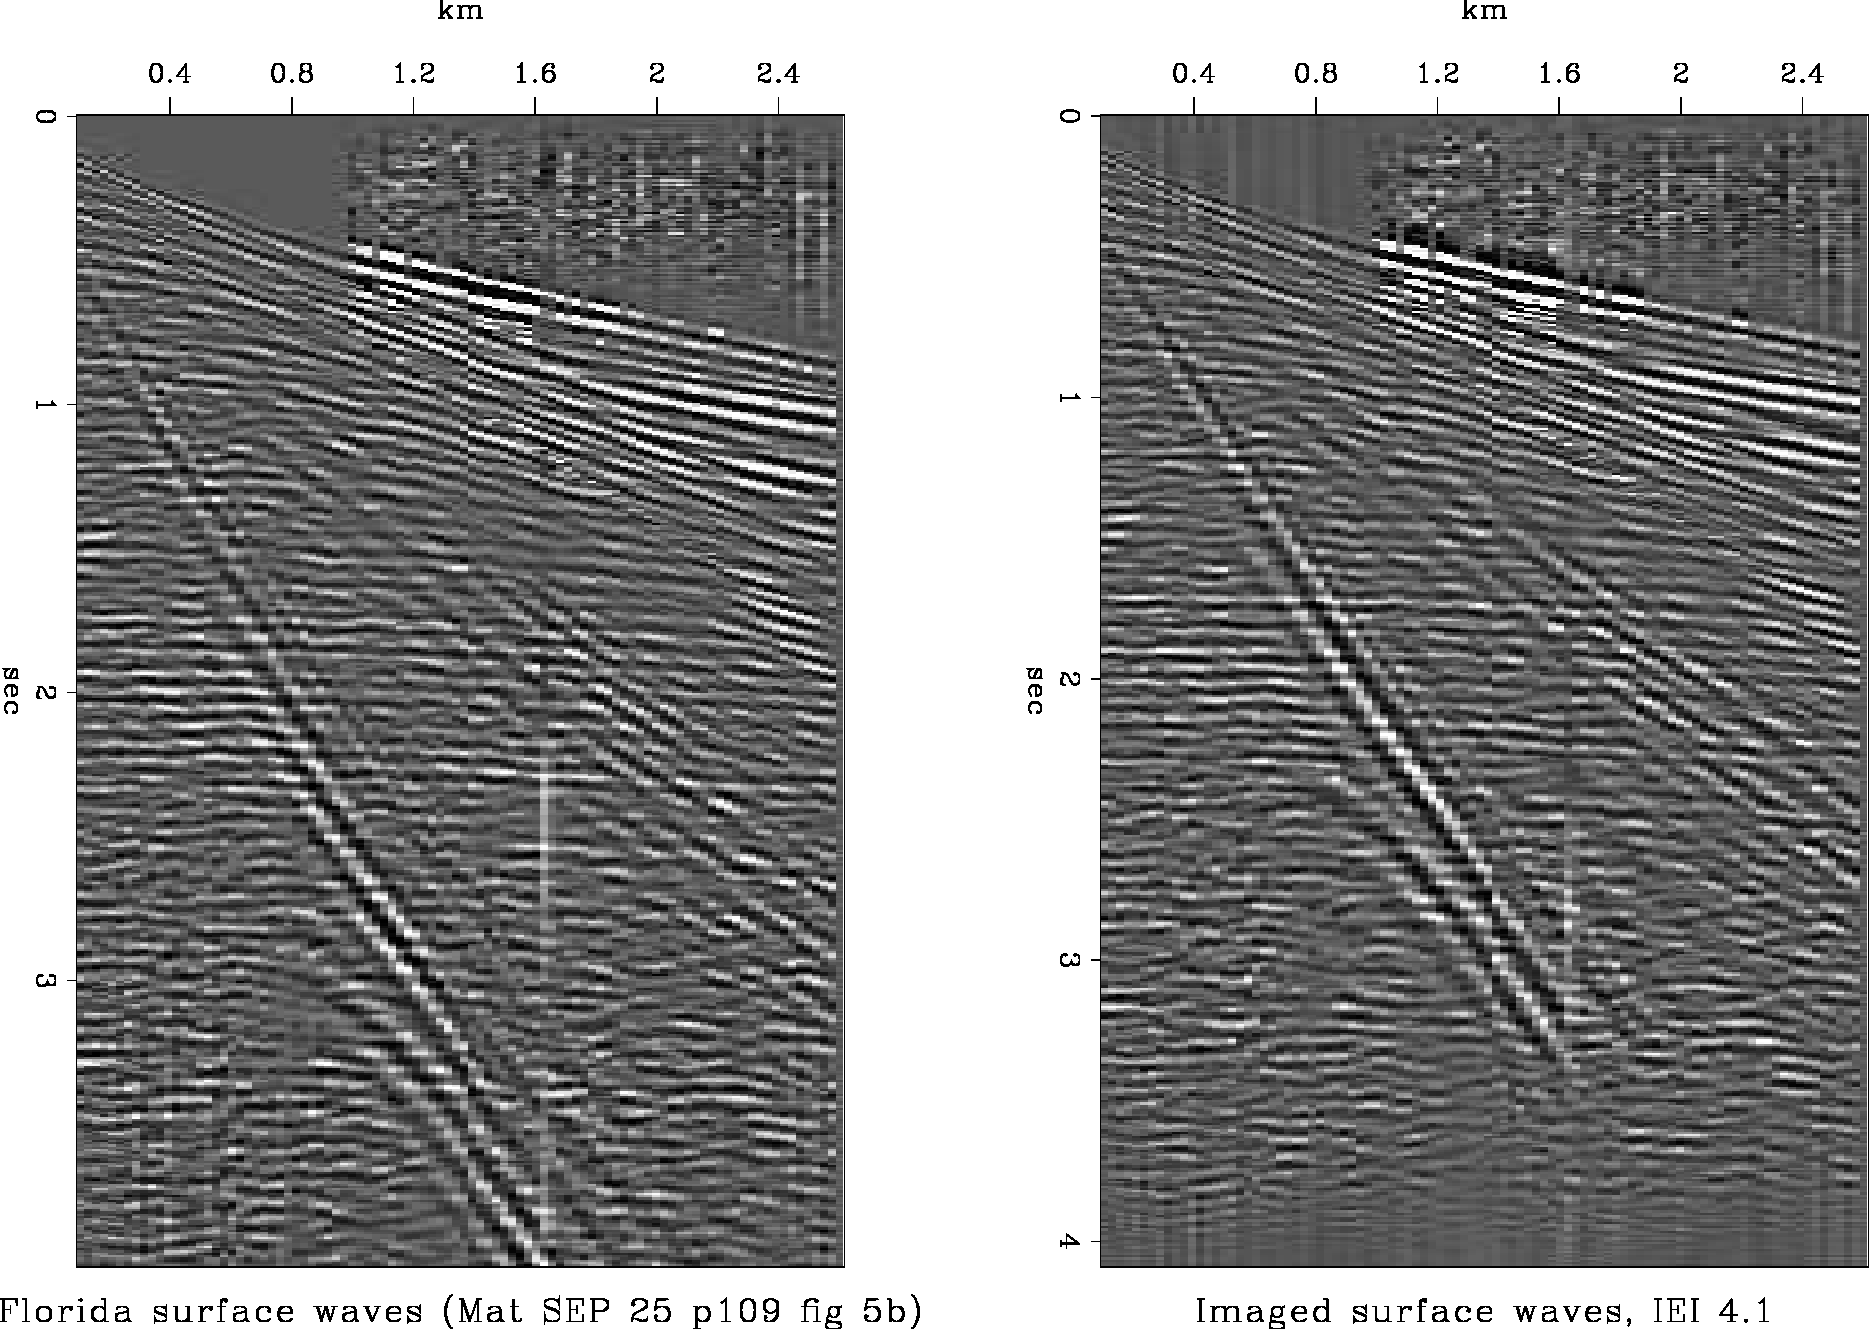
\includegraphics[width=0.65\textwidth]{dspr/sword}
\caption[sword]{频散面波(左图)。消除频散之后(右图)。
图底部表示有两个波至,一是呈直线状的直达波波至,另一是双曲线的一侧,该双曲线必然是由远离测
线之地面上的某种物体所形成的侧反射(据Sword)}
\label{fig:dspr/sword}
\end{figure}

\subsection{偏移剖面上的虚假半圆弧}
\label{sec:4.1.6}

倾角滤波可用于压制多次波。\ref{sec:5.5}节将指出,多次波在一个重要方面是不同于一次波
的:其强度可能沿水平方向作迅速变化。对一次波,必须按绕射双曲线进行扫描偏移,对于
多次波,则不需知此。之所以产生这种差别,是因为对多次波经常得花费很多时间才能聚焦
在不规则近地表区域内。广角偏移剖面的外貌中就包含有类似这种性态的共同特征,这类剖
面往往表现出有许多来自所存路径直至包括来自地表面的半圆弧,这些半圆弧的出现就是警
告我们出了什么差错,半圆弧可能是由多次波、静校正或者无法解释的脉冲干扰所形成。在
许多场合下,都可以局部将它们压制掉而不蝕动到一次波。

\subsection{在倾角空间内消除多次波}
\label{sec:4.1.7}

试将对共深度点叠加结果的偏移看作是在$(\omega,k_x,z)$空间内的向下延拓。一般来
说,速度是随深度而增大的。当向下延拓继续迸行时,速度截止作用沿着指数衰减区的边界
从$(\omega,k_x)$空间中啃掉越来越多的面积(见\ref{sec:1.4}节)。超过这种截止速度的能量是不符合一
次波波动传播模型的,因而一遇到它就要将它压制掉。这样的噪音压制方法可能在较晚的
时间上导致总功率的大大下降。

\subsection{倾角滤波}
\label{sec:4.1.8}

倾角滤波能很方便地同波动外推方程结合起来。我们采用$ik_z=\epsilon-i\omega r_0$。而不是用
$-i\omega r_0$。作初始的Muir展开(参阅\ref{sec:2.1}节,$r_0$是某个准确拟合角度的余弦)。对于15°方程,
我们得
\begin{subequations}
\begin{equation}
ik_z^{15}v=-i\omega+\frac{v^2k_x^2}{\epsilon-i\omega(r_0+1)}
\label{eq:ex4.1.5a}
\end{equation}
对于$45^{\circ}$方程,我们有
\begin{equation}
ik_z^{45}v=-i\omega+\frac{v^2k_x^2}{-2i\omega+\frac{v^2k_x^2}{\epsilon-i\omega(r_0+1)}}
\label{eq:ex4.1.5b}
\end{equation}
\label{eq:ex4.1.5}
\end{subequations}

图\ref{fig:dspr/hyp15}与图\ref{fig:dspr/hyp45}表示15°和45°方程情形下具有倾角滤波参数$\epsilon$及不具有该
参数时的绕射双曲线。

\begin{figure}[H]
\centering
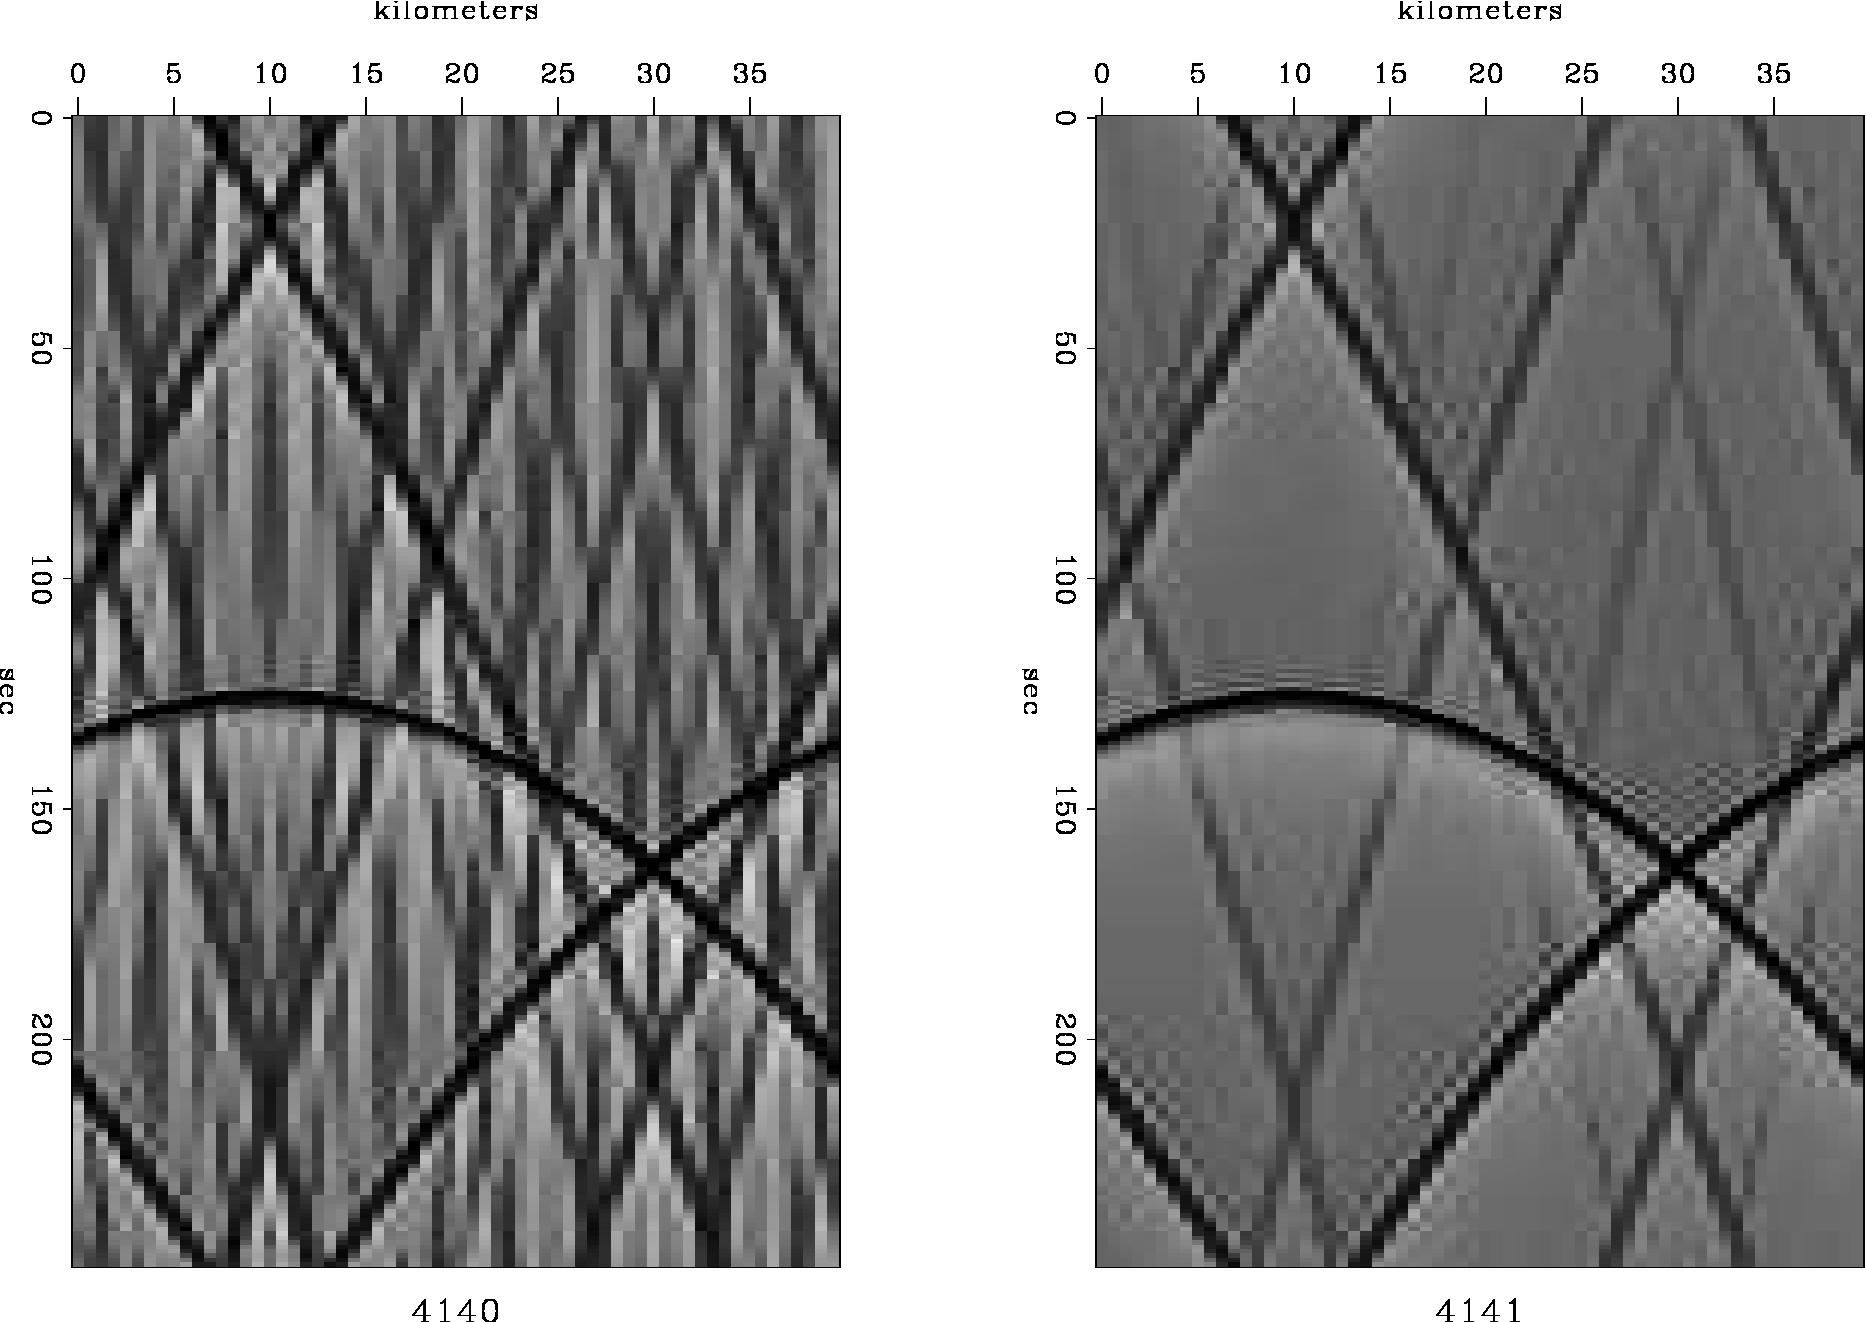
\includegraphics[width=0.65\textwidth]{dspr/hyp15}
\caption[hyp15]{具有倾角滤波(右图)和不带倾角滤波(左图)之15°方程的绕射双曲线}
\label{fig:dspr/hyp15}
\end{figure}

\begin{figure}[H]
\centering
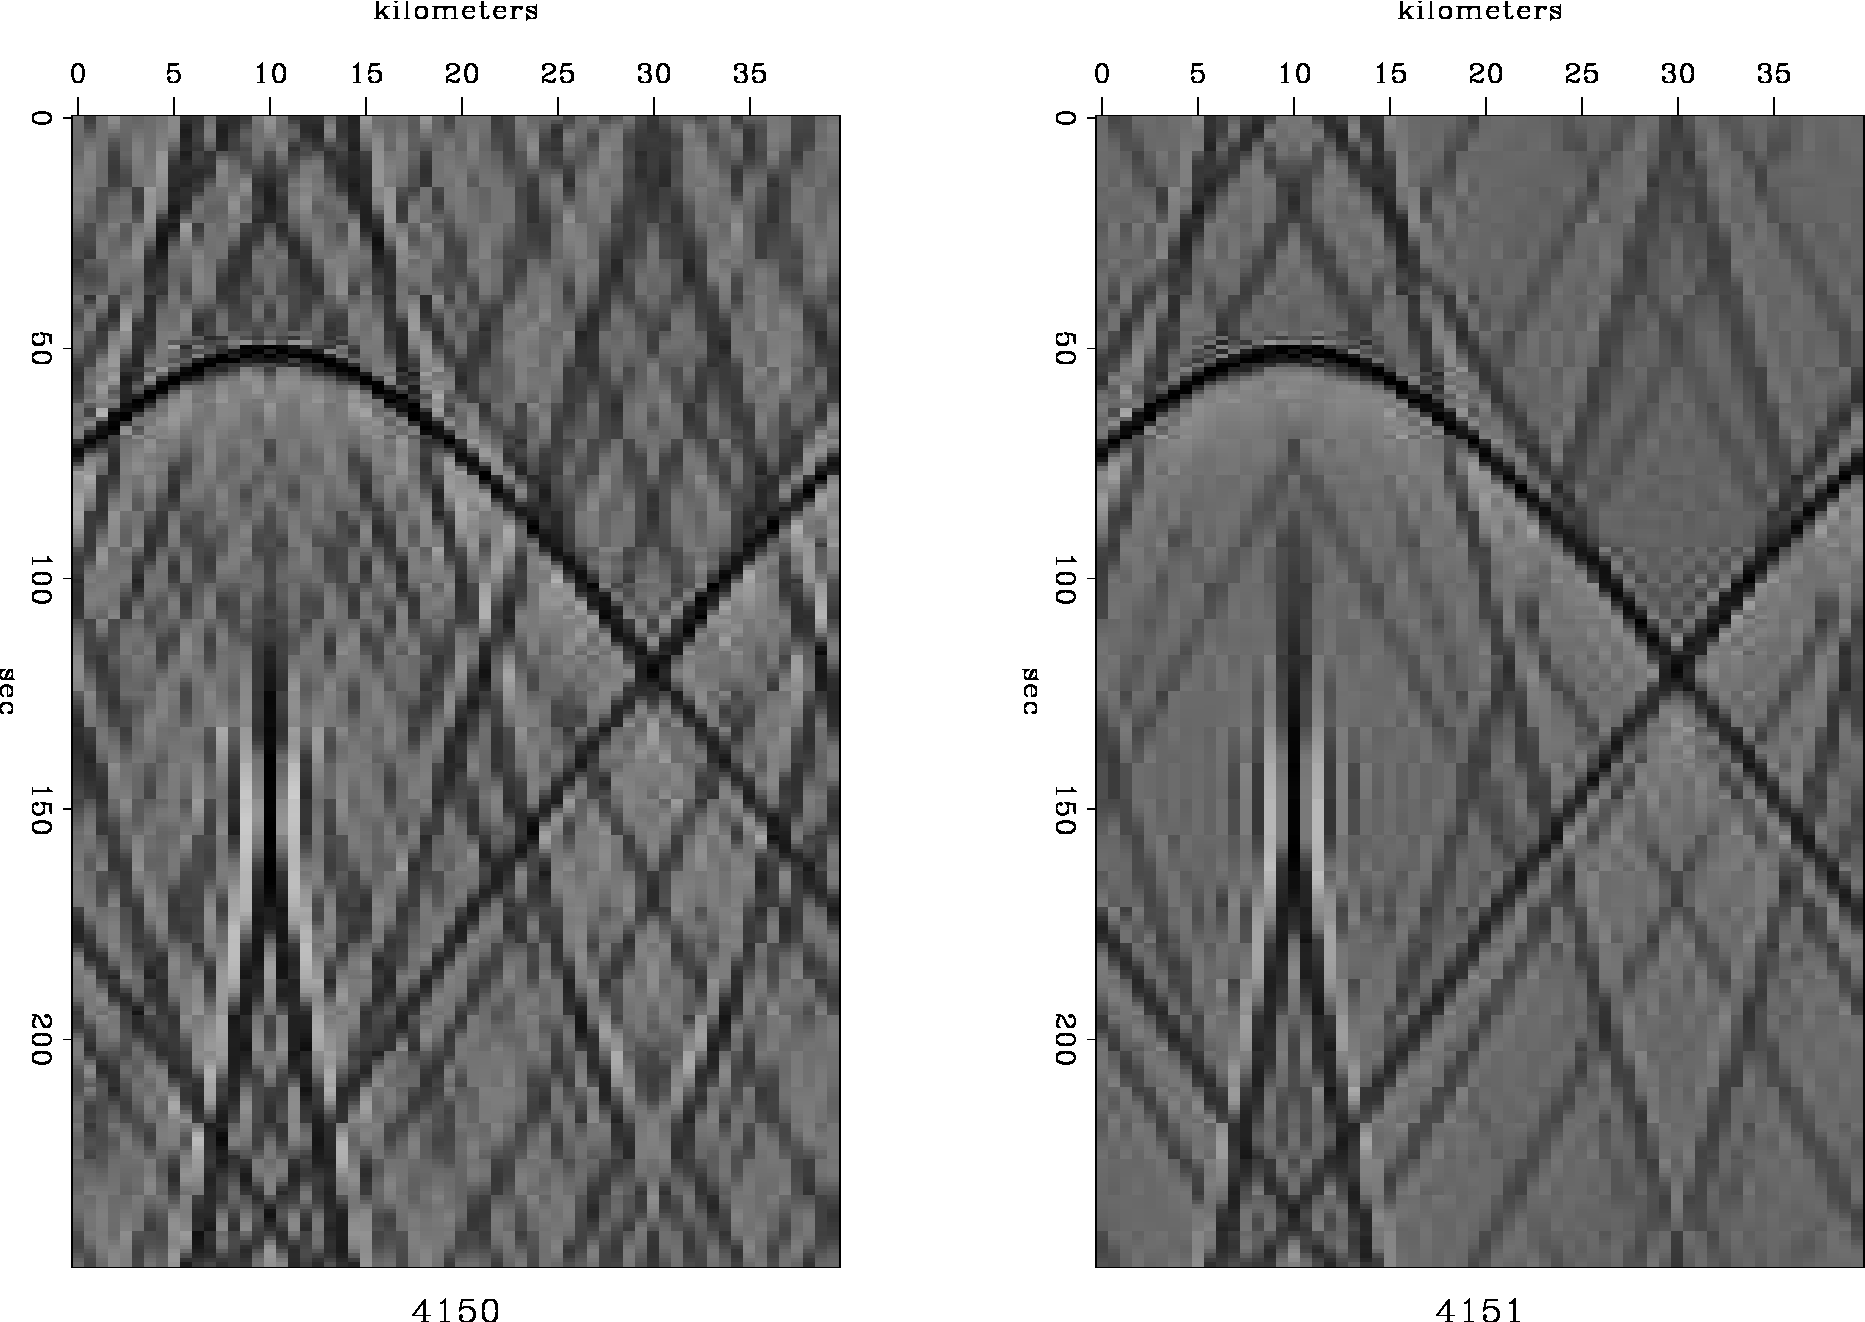
\includegraphics[width=0.65\textwidth]{dspr/hyp45}
\caption[hyp45]{具有倾角滤波(右图)和不带倾角滤波(左图)之45°方程的绕射双曲线}
\label{fig:dspr/hyp45}
\end{figure}

\subsection{倾角滤波资料的混杂面貌}
\label{sec:4.1.9}

对倾角滤波经常提出的一种反对意见是:它可能把资料搞得面貌混杂。混杂的意思是指
各相邻记录道好像都已经加以平均,使得它们不再是独立的了。这确实是倾角滤波的一种影
响,而且由于反射资料水平分辨能力随时间之增大而降低,在较大时间上不可避免炮要出现
这种混杂。横向分辨能力之所以降低,有两个原因:第一,能量猕散引起高频成分消失;第
二,射绣弯曲引起深源的张角(angular aperture)减小(参阅\ref{sec:1.2}节与\ref{sec:1.5}节)。忽视这种基
本限制而幻想各相邻记录道应具有某种独立外貌,那是不现实的。如为了显示的目的而必需
避免混杂,那末,我建议消除低速相干信号生成的噪音而代之以低速非相干的高斯随机噪
音。许多显示装置都是在记录道间距很密时损失动态范围,而随机噪音却可能有助于恢复该
动态范围。

\subsection{使断层显示突出}
\label{sec:4.1.10}

经常能遇到油藏位置受断层控制的情形,但是层状反射面占优势的影响可能掩盖了表示
断层标志的弱绕射波,这时就需要有一种修饰性处理,能够减弱零倾角和小倾角的同相轴,
重点突出10度至60度的倾角范围内之同相轴,然后再将广角反射和指数衰减波能量压制掉。
正如频率滤波的情形一样,是不希望采用锐截止的,因为这意味着脉冲响应会很长(在空间
内,就是脉冲响应很宽)。

\subsection{增益控制也起倾角滤波作用}
\label{sec:4.1.11}

到达时间晚的反射都比到达时间早的反射要弱一些,所以为了显示,普通都利用时变比
例将数据标定。那末,究竟应当是在进行这种按比例标定之前还是在这之后完成偏移呢?答
案将因所感兴趣的方式而有所不同。双曲线顶部有平缓倾角,而到达时间较晚的渐近线则有
陡倾角,因此,放大较晚到达的信息就同放大陡倾角同相轴是完全一致的。我想,选择在比
例标定之前或之后进行偏移,其主要效果也就是最终显示时选择什么倾角谱的问题。过于死
板但正确的作法是,首先迸行偏移,其次进行比例标定,但是这会减弱倾斜同相轴和断层的
信息。而首先进行比例标定,其次进行偏移,则所得结果就比较好一点。后面这种作法有一
个附带的好处,就是采用短字长整数来存贮已经标定过的值,你可以节省计算机内存。在
我的先驱性工作中,我曾采用16位整数存贮,计算与局部存贮采用32位浮点算法。我看很少
有理由要采用现今一般所利用的32位存贮,我们进行记录道之间的内插还不可能达到4位的
精度。

